

Os relatos revelam que, apesar da alta viabilidade operacional indicada pelos indicadores objetivos, a adoção em larga escala depende de \emph{ferramentas de suporte}.   proximo capitulo conclusão e trabalhos futuros

\paragraph{Principais barreiras.}
Os docentes relatam quatro obstáculos centrais:

\begin{enumerate}[label=(\alph*)]
    \item \textbf{Visualização da lógica}: a ausência de uma representação gráfica torna difícil acompanhar onde cada variável é injetada e como as ramificações se desdobram.
    \item \textbf{Falta de modelos-base}: professores novatos no método sentem‐se “sem chão” para iniciar, o que tornou a \emph{Falta de modelos-base prontos} a terceira dificuldade mais citada (4 menções).
    \item \textbf{Sintaxe JSON}: erros simples (vírgulas, chaves) quebram o template inteiro; isso desestimula a exploração manual.
    \item \textbf{Tempo e dependência de IA}: ainda que o ChatGPT acelere o processo, há receio de enviesar o template ou de introduzir erros de concordância.
\end{enumerate}

\paragraph{Sugestões de melhoria.}
Quase todos os participantes convergiram em três frentes:

\begin{enumerate}[label=(\roman*)]
    \item **Interface gráfica em blocos** que permita “arrastar e soltar” condições e variáveis, reduzindo a necessidade de editar JSON cru.
    \item **Pré-visualizador dinâmico** para executar combinações e verificar, em tempo real, a coerência dos enunciados gerados.
    \item **Repositório de templates prontos**, organizado por assunto e nível de dificuldade, servindo como ponto de partida e material de estudo.
\end{enumerate}

\paragraph{Implicações para as Questões de Pesquisa.}
Os relatos revelam que, apesar da alta viabilidade operacional indicada pelos indicadores objetivos, a adoção em larga escala depende de \emph{ferramentas de suporte à autoria}.  Endereçar as três frentes acima pode:

\begin{itemize}
    \item Reduzir o tempo médio de criação de templates (\textbf{QP2});
    \item Aumentar a taxa de reaproveitamento, pois modelos bem estruturados tendem a ser compartilhados (\textbf{QP3});
    \item Mitigar a principal limitação já identificada em QP1—o esforço cognitivo para estruturar ramificações.
\end{itemize}

\begin{figure}[ht]
	\centering
	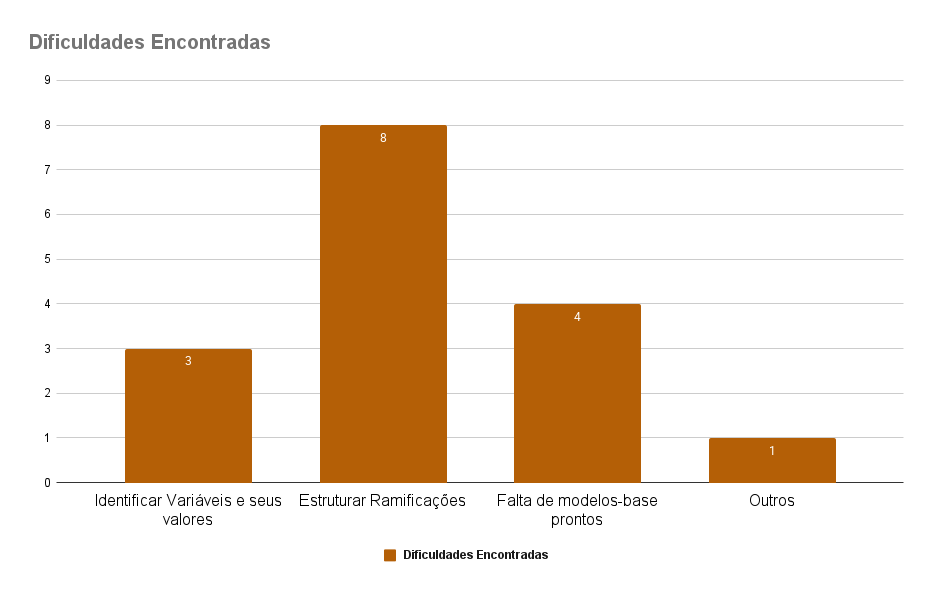
\includegraphics[width=16cm]{./imagens/capitulo8/dificuldades-encontradas}
	\caption{Dificuldades encontradas  (Elaboração própria, 2025) }
	\label{fig:dificuldades-encontradas}
\end{figure}

	

\section{Benefícios e Desafios Percebidos}


O estudo revelou que os professores conseguiram elaborar templates funcionais e diversificados, utilizando as orientações fornecidas. No entanto, alguns desafios foram identificados:

\begin{enumerate}
    \item \textbf{Dificuldade Inicial}: Professores com menor familiaridade com conceitos de questões baseada em templates demonstraram dificuldades em identificar elementos variáveis e combinar os valores.
    \item \textbf{Uso da IA Gnerativa} : A integração do ChatGPT foi bem recebida, e os participantes relataram que as sugestões fornecidas pela ferramenta ajudaram na proposta de contextos diversificados.
    \item \textbf{Percepção Geral} : Os professores consideraram o modelo útil para reduzir o tempo de elaboração de questões, no entanto preferiram que os templates já estivessem prontos pra utilizar, e após construídos pudessem acrescentar ou editar a estrutura conforme a necessidade ao invés de criar do zero.
\end{enumerate}


\begin{table}
\centering

\begin{tabular}{l}
 \\

\end{tabular}

\end{table}

\begin{table}
\centering

\begin{tabular}{l}
\textbf{Resultados} \\

\end{tabular}

\end{table}

\begin{table}
\centering

\begin{tabular}{l}
Quantitativos (tabelas/gráficos) e qualitativos (depoimentos). \\

\end{tabular}

\end{table}

 
\section{Beneficios e Desafios Percebidos} 

redução do esfoço de elaboração, maior diversidade de exercicio

identificar corretamente as variaveis e seus valores
curva de aprendizagem para manipular o template
preferencia em usar templates-base prontos em vez de começar do zero.

\section{Considerações Finais do Estudo de Caso}
A aplicação foi realizada com um número reduzido de professores, o que limita a generalização dos resultados. Estudos futuros poderão expandir o alcance para incluir mais participantes para validar a proposta. Apesar das limitações, a abordagem de geração automática de questões demonstrou um potencial significativo para criar questões em escala e reduzir o esforço necessário para a construção de conteúdos por parte dos professores.


RESPOSTA AS QUESTÕES DE PESQUISA COM OS INDICADORES 
VIABILIDADE : INDICADOR DE TEMPO
UTILIDADE : TAXA DE APROVEITAMENTO 
DESAFIOS : FALTA DE MODELOS PRÉ-PRONTOS

AMOSTRA REDUZIDA LIMITA A GENERALIZAÇÃO

----- CONTINUE AQUOI ---  PARE AQUIIII


\subsubsection{\textbf{Resultados}}

\paragraph{\textbf{7.8.1 Eficiência do processo}}

Tempo médio para criar o primeiro template: 27 min (desvio-padrão 6,2 min). Média de 12,4 questões por template e reaproveitamento de 83 \%.

\paragraph{\textbf{7.8.2 Depoimentos dos professores}}

\begin{quote}
“Com o guia, consegui transformar rapidamente uma questão antiga em um template; a IA me ajudou a criar três variações de contexto em minutos.” — P2

\end{quote}

\paragraph{\textbf{7.8.3 Benefícios percebidos}}

Redução do esforço de elaboração, maior diversidade de exercícios e incremento no engajamento dos alunos.

\paragraph{\textbf{7.8.4 Desafios e dificuldades}}

\begin{itemize}
    \item Identificar corretamente as variáveis e seus valores.
    \item Curva de aprendizagem para manipular placeholders.
    \item Preferência por templates-base prontos em vez de começar do zero.
\end{itemize}
 

\paragraph{\textbf{Principais Desafios Identificados}}

\begin{itemize}
    \item \textbf{Curva de aprendizagem inicial} (especialmente na identificação de variáveis e condições);
    \item \textbf{Necessidade de modelos‐base} para acelerar a adoção;
    \item \textbf{Integração com sistemas de avaliação existentes} (Moodle, Google Forms, etc.), que exigirá conversores automáticos — apontado como trabalho futuro.
\end{itemize}
\textbf{QP3 – Desafios:} maior dificuldade em definir variáveis e preferências por templates‐base prontos; 60 \% solicitaram um repositório inicial de modelos. 


Síntese interpretativa
Em conjunto, os três gráficos indicam que:

Viabilidade: a mediana de ~30 min coloca a criação de templates dentro de um tempo aceitável para reuniões de planejamento.

Eficiência: gerar entre 10 e 15 questões a partir de um único template demonstra economia de esforço na produção de exercícios.

Reutilização: a taxa de sucesso plena na conversão de questões reais comprova que o método não exige partir do zero, favorecendo adoção incremental.


Endereçar as três frentes acima pode:

\begin{itemize}
    \item Reduzir o tempo médio de criação de templates (\textbf{QP2});
    \item Aumentar a taxa de reaproveitamento, pois modelos bem estruturados tendem a ser compartilhados (\textbf{QP3});
    \item Mitigar a principal limitação já identificada em QP1—o esforço cognitivo para estruturar ramificações.
\end{itemize}
